\section{Platform comparing}
In order to implement the previous discussed effects digitally, a platform has to be chosen. In this section a list of possible platforms for the effect implementation will be analysed. The following platforms will be analysed:

\begin{itemize}
\item Rasperry pi
\item \gls{dsp}
\item \gls{fpga}
\end{itemize}

\subsection{Raspberry pi}
There exist different generations of the Raspberry pi, but the one that will be analysed is the Raspberry pi 3 model B, since it is the latest version. 
A Raspberry pi is a \gls{sbc} at the size of a credit-card. A picture of the Raspberry pi 3 model B, is shown in \autoref{fig:RP3mB}.

\begin{figure}[h]
	\centering
		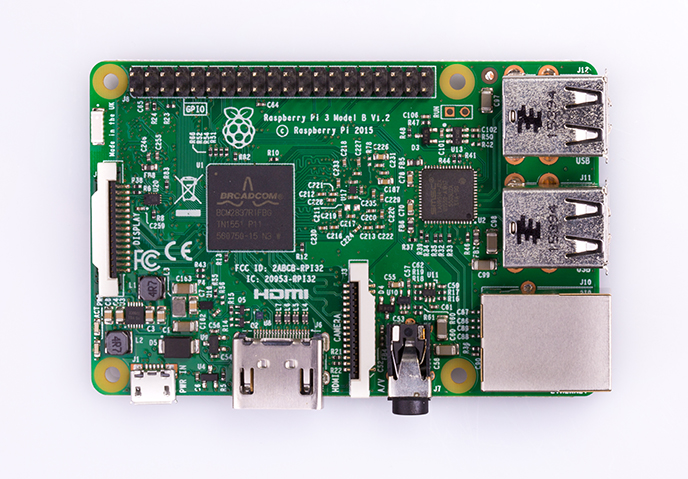
\includegraphics[width=0.7\textwidth]{Raspberry_pi_3_model_B.jpg}
		\caption{Picture of the Raspberry Pi 3 model B \cite{Raspberry_pi}.}
		\label{fig:RP3mB}
\end{figure}

The Raspberry pi 3 model B has a 1.2 GHz Quad-core ARM processor, supports wireless LAN and Bluetooth 4.1. It has 1GB RAM and has connectors for micro SD cards \cite{Raspberry_pi}.
The Raspberry Pi is Linux based, but can also run Windows \cite{sparkfun_Raspberry_pi}. This makes the Raspberry pi 3 model B suited for a wide range of projects. This is both its advantage and its disadvantage if a specialized platform is wanted. 

\subsection{Digital Signal Processor}
A \gls{dsp} is a processor, which is optimized for high-speed numerical operations such as: Addition, subtraction and multiplication. A typical \gls{dsp} system includes an anti-aliasing filter, an \gls{adc}, a \gls{dsp}, a host interface, a \gls{dac} and a anti-imaging filter. A block diagram of the typical \gls{dsp} system is shown in \autoref{fig:typ_dsp}.

\begin{figure}
\centering
\def\svgwidth{\columnwidth}
\input{figures/analysing/DSP_typical.pdf_tex}
\caption{Block diagram of a typical \gls{dsp} \cite{AnalogDialogue}.}
		\label{fig:typ_dsp}
\end{figure}

These high-speed numerical operations make the \gls{dsp} suited for real-time applications, and a \gls{dsp} can work both as a sample-based system and as a frame-based system. 
Two terms are commonly used for describing the processing power of a \gls{dsp}. These are \gls{mips} and \gls{mops}. The requirements of the \gls{dsp} can be found, based on the sampling interval and the number of operations needed between each sample. This is shown in \eqref{eq:MOPS}.

\begin{equation}\label{eq:MOPS}
        DSP_{speed} = \frac{Operations}{T_s}\addunit{MOPS}
    \end{equation}

    \startexplain
        \explain{$DSP_{speed}$ is the \gls{dsp}'s processing power}{MOPS}
        \explain{$Operations$  is the number of operations}{1}
        \explain{$T_s$ is the sampling interval}{\si{\second}}
    \stopexplain


\gls{mips} and \gls{mops} are not the same, but related in the way that each \gls{dsp} instruction containe a numbers for operation  \cite{AnalogDialogue}. E.g. a \gls{dsp} with 4 \gls{mips} and 8 \gls{mops} means that the \gls{dsp} can preform 2 operation for each instruction.


